% !TeX root = ../main.tex
\section{Phương pháp đề xuất}
\label{sec:proposed_method}

Nghiên cứu xây dựng một họ phương pháp dựa trên
\textbf{TransReID}~\cite{he2021transreidtransformerbasedobjectreidentification}
với mục tiêu khai thác thông tin nhìn thấy ở mức patch nhằm cải thiện chất
lượng biểu diễn cho bài toán Person ReID. Giả thuyết là không phải mọi patch đều đóng góp như nhau vào đặc trưng cuối
cùng: các patch chứa vùng người ổn định, ít bị che khuất và giàu thông tin
nhận dạng cần được ưu tiên hơn so với các patch nền hoặc patch nhiễu. Trên cơ
sở đó, nghiên cứu bổ sung vào pipeline của TransReID một nhánh dự đoán trọng số
nhìn thấy cho từng patch, sau đó khảo sát nhiều chiến lược tích hợp khác nhau,
từ thay thế trực tiếp, hợp nhất tuyến tính cho đến hiệu chỉnh residual có kiểm
soát.

\subsection{Tổng quan kiến trúc}

Ảnh đầu vào trước hết được chia thành các patch và được đưa qua backbone
Transformer của TransReID để thu được tập patch embeddings cùng đặc trưng toàn
cục. Trên không gian đặc trưng này, một nhánh phụ được thêm vào nhằm ước lượng
mức độ hữu ích của từng patch đối với nhiệm vụ truy hồi. Các trọng số thu được
không thay đổi backbone gốc, mà được sử dụng để xây dựng một đặc trưng phụ trợ
phản ánh phần thông tin nhìn thấy đáng tin cậy hơn. Tùy theo từng biến thể thực
nghiệm, đặc trưng phụ trợ này sẽ được sử dụng theo các cách khác nhau để hình
thành đặc trưng truy hồi cuối cùng.

Hình~\ref{fig:two_pipelines} minh họa đồng thời pipeline baseline và pipeline
mở rộng để làm rõ vị trí của nhánh \textit{visibility-guided patch weighting}
trong kiến trúc tổng thể.

\begin{figure*}[!t]
    \centering
    \begin{minipage}[t]{0.48\textwidth}
        \centering
        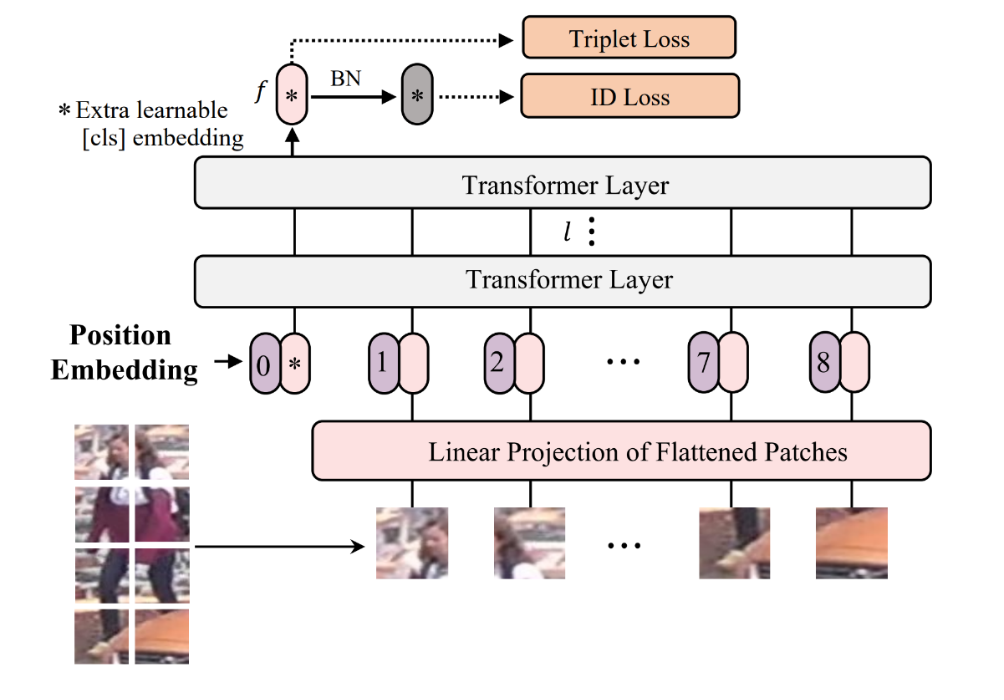
\includegraphics[width=\linewidth]{figures/pipeline.png}

        \vspace{2pt}
        \small (a) Pipeline baseline
    \end{minipage}
    \hfill
    \begin{minipage}[t]{0.48\textwidth}
        \centering
        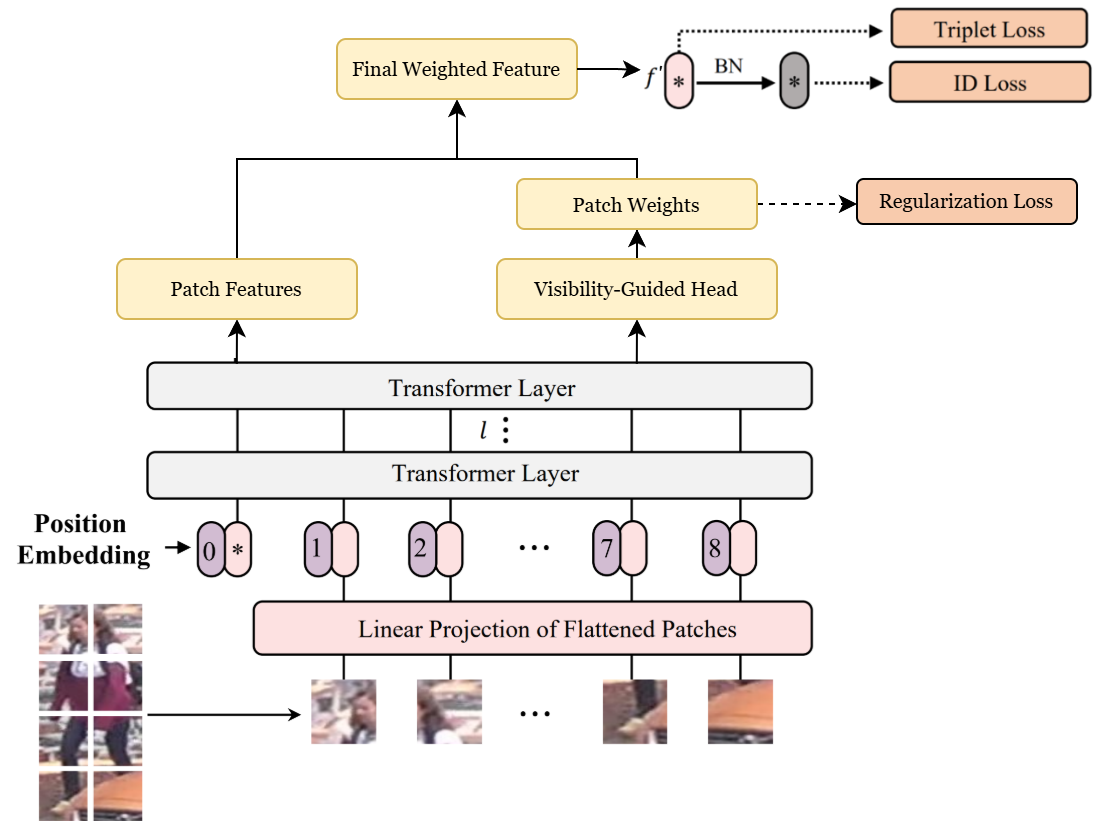
\includegraphics[width=\linewidth]{figures/new_pipeline.png}

        \vspace{2pt}
        \small (b) Pipeline đề xuất với visibility-guided patch weighting
    \end{minipage}
    \caption{So sánh giữa pipeline TransReID gốc và pipeline mở rộng với nhánh
    ước lượng trọng số theo patch.}
    \label{fig:two_pipelines}
\end{figure*}

\subsection{Mô hình hóa trọng số nhìn thấy ở mức patch}

Ký hiệu \(Z=[z_1,z_2,\dots,z_N]\), với \(z_i \in \mathbb{R}^{d}\), là tập patch
embeddings được trích xuất từ backbone. Để lượng hóa tầm quan trọng của từng
patch, nghiên cứu bổ sung một đầu dự đoán nhẹ dưới dạng MLP, cho đầu ra là
trọng số nhìn thấy \(w_i\):
\[
w_i = \sigma(\mathrm{MLP}(z_i)),
\]
trong đó \(\sigma(\cdot)\) là hàm sigmoid. Trọng số lớn hơn tương ứng với patch
được xem là chứa nhiều thông tin hữu ích hơn cho nhận dạng.

Từ các trọng số này, một đặc trưng phụ trợ dựa trên patch được xây dựng thông
qua phép tổng hợp có trọng số:
\[
f_{\mathrm{vis}} = \frac{\sum_{i=1}^{N} w_i z_i}{\sum_{i=1}^{N} w_i + \epsilon},
\]
trong đó \(\epsilon\) là hằng số nhỏ nhằm tránh chia cho \(0\). Cách biểu diễn
này cho phép mô hình tập trung mạnh hơn vào các vùng đáng tin cậy, đồng thời
giảm ảnh hưởng của các patch bị che khuất hoặc chứa nền.

\subsection{Các chiến lược tích hợp đặc trưng}

Thay vì giả định duy nhất một cách kết hợp giữa đặc trưng toàn cục gốc và đặc
trưng phụ trợ theo patch, nghiên cứu khảo sát một họ chiến lược tích hợp. Trong
biến thể hợp nhất tuyến tính, đặc trưng cuối cùng được xác định bởi
\[
f_{\mathrm{final}} = \alpha f_{\mathrm{global}} + (1-\alpha) f_{\mathrm{vis}},
\]
với \(f_{\mathrm{global}}\) là đặc trưng toàn cục của TransReID và
\(\alpha \in [0,1]\) là hệ số điều khiển mức đóng góp của nhánh mới. Thiết kế
này cho phép bảo toàn lợi thế của biểu diễn global gốc mà vẫn khai thác
thông tin từ các patch có độ tin cậy cao.

Đối với các cấu hình được huấn luyện từ khởi tạo ImageNet, nghiên cứu còn khảo
sát một dạng tích hợp bảo thủ hơn dưới dạng hiệu chỉnh residual:
\[
f_{\mathrm{final}} = f_{\mathrm{global}} + \gamma \cdot
\bigl(f_{\mathrm{vis}} - f_{\mathrm{global}}\bigr),
\]
trong đó \(\gamma\) là hệ số cổng học được. Cơ chế này bảo đảm nhánh mới chỉ
điều chỉnh biểu diễn gốc một cách từ từ, nhờ đó làm quá trình tối ưu ổn định
hơn khi mô hình chưa mang sẵn tri thức ReID chuyên biệt.

Ngoài hai chiến lược chính nêu trên, các thực nghiệm cũng khảo sát những biến
thể khác như áp dụng weighting trên các nhánh local của JPM, lọc
\textit{foreground-aware top-k patches}, hoặc mở rộng pipeline bằng \textit{token enrichment} và
\textit{synthetic occlusion augmentation}. Các biến thể này không thay đổi giả thuyết cơ
sở của phương pháp, mà đóng vai trò khảo sát mức độ phù hợp của từng cách tích
hợp trong những điều kiện khởi tạo khác nhau.

\subsection{Hợp nhất token theo độ quan sát có xét che khuất (OVTF)}

Trong nhóm cấu hình được huấn luyện từ khởi tạo ImageNet, nghiên cứu lựa chọn
một biến thể \textbf{Occlusion-aware Visibility-guided Token Fusion}
(OVTF), nhằm kết hợp cơ chế
gán trọng số theo độ quan sát với các thành phần tăng cường biểu diễn và tăng
độ bền vững trước che khuất. OVTF vẫn giữ backbone TransReID kết hợp JPM, đồng
thời kết hợp bốn thành phần bổ trợ theo một pipeline thống nhất. Trước hết,
\textbf{visibility-guided patch weighting} gán cho mỗi patch token một trọng số
nhìn thấy thông qua một đầu dự đoán nhẹ nhằm lượng hóa mức độ hữu ích của vùng
đó đối với truy hồi. Trên cơ sở các trọng số này, cơ chế
\textbf{dynamic top-k token enrichment} chọn ra nhóm patch có độ tin cậy cao
nhất để xây dựng một \textit{visible prototype}, rồi sử dụng prototype đó để
tăng cường trở lại cho toàn bộ patch token trước khi tổng hợp đặc trưng. Ở pha
suy luận, \textbf{JPM fusion} ghép đặc trưng từ nhánh toàn cục với bốn nhánh cục
bộ của JPM nhằm đồng thời duy trì thông tin toàn cục và chi tiết vùng. Cuối
cùng, \textbf{synthetic occlusion augmentation} bổ sung các mẫu che khuất tổng
hợp trong quá trình huấn luyện để tăng độ bền vững của mô hình trong điều kiện che khuất
và hỗ trợ duy trì tính nhất quán của biểu diễn đặc trưng.

Gọi \(\mathrm{TopK}\) là tập các patch có trọng số cao nhất, prototype được
xây dựng như sau:
\[
p = \sum_{i \in \mathrm{TopK}} \alpha_i z_i,
\qquad
\alpha_i = \frac{\exp(w_i)}{\sum_{j \in \mathrm{TopK}} \exp(w_j)}.
\]
Prototype này sau đó được dùng để tăng cường trở lại cho patch embeddings:
\[
\tilde{z}_i = z_i + \lambda w_i p.
\]
Từ các patch đã được tăng cường, đặc trưng phụ trợ mới được tổng hợp bởi
\[
f_{\mathrm{aug}} = \frac{\sum_i w_i \tilde{z}_i}{\sum_i w_i + \epsilon}.
\]
Thiết kế trên cho phép nhánh patch-level không chỉ làm nhiệm vụ đánh trọng số,
mà còn lan truyền thông tin từ các vùng có độ tin cậy cao đến toàn bộ biểu
diễn. Trong pha suy luận, \(f_{\mathrm{aug}}\) được sử dụng cùng nhánh toàn cục
và các nhánh cục bộ JPM để hình thành đặc trưng truy hồi cuối cùng.

Về tối ưu hóa, OVTF kế thừa cơ chế \textit{softmax + soft triplet} của
TransReID trên nhánh toàn cục và các nhánh JPM. Để tránh phân phối trọng số
theo patch bị suy biến, hàm mục tiêu được bổ sung một thành phần điều chuẩn
\(\mathcal{L}_{reg}\). Khi áp dụng tăng cường che khuất tổng hợp, hàm mục tiêu
tiếp tục được mở rộng bởi hai thành phần \(\mathcal{L}_{occ}\) và
\(\mathcal{L}_{cons}\), tương ứng dùng để tăng khả năng nhận dạng trên các mẫu
bị che khuất và ràng buộc tính nhất quán giữa ảnh gốc với ảnh che khuất tổng
hợp. Khi đó, hàm mất mát tổng quát có thể được viết dưới dạng:
\[
\mathcal{L}
= \mathcal{L}_{ID}^{JPM}
+ \mathcal{L}_{tri}^{JPM}
+ \lambda_{\mathrm{reg}}\mathcal{L}_{reg}
+ \lambda_{\mathrm{occ}}\mathcal{L}_{occ}
+ \lambda_{\mathrm{cons}}\mathcal{L}_{cons}.
\]
Trong đó, \(\mathcal{L}_{reg}\) giúp phân phối trọng số nhìn thấy giữ được tính
phân biệt, \(\mathcal{L}_{occ}\) tăng khả năng nhận dạng khi một phần cơ thể bị
che khuất, còn \(\mathcal{L}_{cons}\) ép biểu diễn của cặp (ảnh gốc, ảnh bị
che) không lệch nhau quá xa trong không gian đặc trưng. Các siêu tham
số chi tiết của cấu hình OVTF được trình bày tại
Phụ lục~\ref{sec:appendix_experimental_config}.
